\newcommand{\svcourse}{CST Part IA: Introduction to Probability}
\newcommand{\svnumber}{1}
\newcommand{\svvenue}{Churchill, Room TBD}
\newcommand{\svdate}{2022-05-14}
\newcommand{\svtime}{11:00}
\newcommand{\svuploadkey}{PO5ogKIM8KQA22FZS8IAf8gxA8XKi19jxIBVHIfFZ+3GCBXuNUXS9lVN6bNYjxM/}

\newcommand{\svrname}{Mr Matthew Ireland}
\newcommand{\jkfside}{twoside}
\newcommand{\jkfhanded}{right}

\newcommand{\studentname}{Harry Langford}
\newcommand{\studentemail}{hjel2@cam.ac.uk}


\documentclass[10pt,\jkfside,a4paper]{article}

% DO NOT add \usepackage commands here.  Place any custom commands
% into your SV work files.  Anything in the template directory is
% likely to be overwritten!

\usepackage{fancyhdr}

\usepackage{lastpage}       % ``n of m'' page numbering
\usepackage{lscape}         % Makes landscape easier

\usepackage{verbatim}       % Verbatim blocks
\usepackage{epsfig}         % Embed encapsulated postscript
\usepackage{array}          % Array environment
\usepackage[nolinks]{qrcode}         % QR codes
\usepackage{enumitem}       % Required by Tom Johnson's exam question header

\usepackage{hhline}         % Horizontal lines in tables
\usepackage{siunitx}        % Correct spacing of units
\usepackage{amsmath}        % American Mathematical Society
\usepackage{amssymb}        % Maths symbols
\usepackage{amsthm}         % Theorems

\usepackage{ifthen}         % Conditional processing in tex

\usepackage[top=3cm,
            bottom=3cm,
            inner=2cm,
            outer=5cm]{geometry}

% PDF metadata + URL formatting
\usepackage[
            pdfauthor={\studentname},
            pdftitle={\svcourse, SV \svnumber},
            pdfsubject={},
            pdfkeywords={9d2547b00aba40b58fa0378774f72ee6},
            pdfproducer={},
            pdfcreator={},
            hidelinks]{hyperref}

\renewcommand{\headrulewidth}{0.4pt}
\renewcommand{\footrulewidth}{0.4pt}
\fancyheadoffset[LO,LE,RO,RE]{0pt}
\fancyfootoffset[LO,LE,RO,RE]{0pt}
\pagestyle{fancy}
\fancyhead{}
\fancyhead[LO,RE]{{\bfseries \studentname}\\\studentemail}
\fancyhead[RO,LE]{{\bfseries \svcourse, SV~\svnumber}\\\svdate\ \svtime, \svvenue}
\fancyfoot{}
\fancyfoot[LO,RE]{For: \svrname}
\fancyfoot[RO,LE]{\today\hspace{1cm}\thepage\ / \pageref{LastPage}}
\fancyfoot[C]{\qrcode[height=0.8cm]{\svuploadkey}}
\setlength{\headheight}{22.55pt}

\ifthenelse{\equal{\jkfside}{oneside}}{

 \ifthenelse{\equal{\jkfhanded}{left}}{
  % 1. Left-handed marker, one-sided printing or e-marking, use oneside and...
  \evensidemargin=\oddsidemargin
  \oddsidemargin=73pt
  \setlength{\marginparwidth}{111pt}
  \setlength{\marginparsep}{-\marginparsep}
  \addtolength{\marginparsep}{-\textwidth}
  \addtolength{\marginparsep}{-\marginparwidth}
 }{
  % 2. Right-handed marker, one-sided printing or e-marking, use oneside.
  \setlength{\marginparwidth}{111pt}
 }

}{
 % 3. Alternating margins, two-sided printing, use twoside.
}

\setlength{\parindent}{0em}
\addtolength{\parskip}{1ex}

% Exam question headings, labels and sensible layout (courtesy of Tom Johnson)
\setlist{parsep=\parskip, listparindent=\parindent}
\newcommand{\examhead}[3]{\section{#1 Paper #2 Question #3}}
\newenvironment{examquestion}[3]{
    \examhead{#1}{#2}{#3}\setlist[enumerate, 1]{label=(\alph*)}\setlist[enumerate, 2]{label=(\roman*)}
    \marginpar{\qrcode{https://www.cl.cam.ac.uk/teaching/exams/pastpapers/y#1p#2q#3.pdf}}
    \marginpar{\footnotesize \url{https://www.cl.cam.ac.uk/teaching/exams/pastpapers/y#1p#2q#3.pdf}}
}{}



\usepackage{tikz}
\usepackage{mathtools}
\usepackage{xcolor}

\definecolor{colour1}{RGB}{254, 0, 0}
\definecolor{colour2}{RGB}{247, 72, 17}
\definecolor{colour3}{RGB}{239, 103, 30}
\definecolor{colour4}{RGB}{230, 127, 40}
\definecolor{colour5}{RGB}{220, 148, 48}
\definecolor{colour6}{RGB}{209, 167, 56}
\definecolor{colour7}{RGB}{196, 185, 61}
\definecolor{colour8}{RGB}{178, 204, 61}
\definecolor{colour9}{RGB}{151, 223, 54}
\definecolor{colour10}{RGB}{98, 243, 33}

\usepackage[T1]{fontenc}

\usepackage{textcomp}

\lstset{language=Python, upquote=true}

\begin{document}

\section{Genome Sequencing}

\begin{enumerate}

    \item From a high level, explain the problem of \textit{genome sequencing}, and what are the given inputs and desirable outputs. What limitations prevent us from having more informative inputs?

    Genome sequencing is the problem of extracting the genome of a cell from a collection of reads. We start by taking a set of white blood cells (containing many copies of DNA), immerse them in a denaturing agent
    to break it down into small strands. We then read some of the first characters of them: these are called reads. Each read is roughly 100--400 bases long. The bioinformatics problem of Genome Sequencing
    arises from taking these reads and reconstructing the original genome.

    The inputs to the algorithm are a multiset of $k$-mers -- defined as the (disjoint) union of all subsequences of length $k$ in any read. The desired outputs is the genome which is most likely to have
    generated such an output.

    We can't get a more informative input because sequencing machines are unable to read sufficiently long sequences. For example the length of Chromosome 1 in humans is 100 million bases.

    \item Define a $k$-mer, a \textit{prefix} and a \textit{suffix} of a string within this context. How are these individual components used within the Hamiltonian and de Bruijn graphs?

    A k-mer is a sequence of k bases. A prefix is the first $k - 1$ bases in a $k$-mer. A suffix is the last $k - 1$ bases in a $k$-mer.

    \item What is a necessary condition for a graph to have a Eulerian cycle?

    Every node has both an even in-degree and an even out-degree.

    \item There exists an $\mathcal O(n^2 2^n)$-time algorithm for computing Hamiltonian paths (where $n$ is the number of nodes). Conversely, what is the computational complexity of the best-known algorithm for
    computing Eulerian cycles? Provide pseudocode for both of those algorithms.

    The complexity of finding a Hamiltonian Cycle is $\mathcal O(n^2 \cdot 2^n)$ and is a brute force algorithm.

    \lstinputlisting{hamiltonian.py}

    The complexity of finding an Eulerian Cycle is $\mathcal O(n)$ for a graph with $n$ edges.

    \lstinputlisting{eulerian.py}

    \item Build the Hamiltonian and de Bruijn graphs over the following set of $k$-mers: \texttt{\{"ATG", "TGG", "GGC", "GCG", "CGT", "GTG", "TGC", "GCA", "CAA", "AAT"\}}

    \begin{figure}[H]

        \centering

        \begin{tikzpicture}

            \node (atg) at (0, 0) {\texttt{ATG}};
            \node (tgg) at (1.5, 0) {\texttt{TGG}};
            \node (ggc) at (3, 0) {\texttt{GGC}};
            \node (gcg) at (4.5, 0) {\texttt{GCG}};
            \node (cgt) at (6, 0) {\texttt{CGT}};
            \node (gtg) at (7.5, 0) {\texttt{GTG}};
            \node (tgc) at (9, 0) {\texttt{TGC}};
            \node (gca) at (10.5, 0) {\texttt{GCA}};
            \node (caa) at (12, 0) {\texttt{CAA}};
            \node (aat) at (13.5, 0) {\texttt{AAT}};

            \draw [-stealth, red] (atg) -- (tgg);
            \draw [-stealth, red] (tgg) -- (ggc);
            \draw [-stealth, red] (ggc) -- (gcg);
            \draw [-stealth, red] (gcg) -- (cgt);
            \draw [-stealth, red] (cgt) -- (gtg);
            \draw [-stealth, red] (gtg) -- (tgc);
            \draw [-stealth, red] (tgc) -- (gca);
            \draw [-stealth, red] (gca) -- (caa);
            \draw [-stealth, red] (caa) -- (aat);

            \path [-stealth, bend left] (atg) edge (tgc);
            \path [-stealth, bend left] (ggc) edge (gca);
            \path [-stealth, bend left] (gtg) edge (tgg);
            \path [-stealth, bend left] (tgc) edge (gcg);
            \path [-stealth, bend left] (aat) edge (atg);

        \end{tikzpicture}

        \caption{Hamiltonian Graph}

    \end{figure}

    \begin{figure}[H]

       \centering

        \begin{tikzpicture}

            \node (at) at (0.0, 0) {\texttt{AT}};
            \node (tg) at (1.5, 0) {\texttt{TG}};
            \node (gg) at (3.0, 0) {\texttt{GG}};
            \node (gc) at (4.5, 0) {\texttt{GC}};
            \node (cg) at (6.0, 0) {\texttt{CG}};
            \node (gt) at (7.5, 0) {\texttt{GT}};
            \node (ca) at (9.0, 0) {\texttt{CA}};
            \node (aa) at (10.5, 0) {\texttt{AA}};

            \path [-stealth, colour1] (at) edge (tg);
            \path [-stealth, colour2] (tg) edge (gg);
            \path [-stealth, colour3] (gg) edge (gc);
            \path [-stealth, colour4] (gc) edge (cg);
            \path [-stealth, colour5] (cg) edge (gt);
            \path [-stealth, colour9] (ca) edge (aa);

            \path [-stealth, bend left, colour6] (gt) edge (tg);
            \path [-stealth, bend left, colour10] (aa) edge (at);
            \path [-stealth, bend left, colour7] (tg) edge (gc);
            \path [-stealth, bend left, colour8] (gc) edge (ca);

        \end{tikzpicture}

        \caption{De Bruijn Graph}

    \end{figure}

    \item Explain how to sequence a genome using de Bruijn graphs constructed from \textit{paired reads}. What is the limitation of the previous approach to sequencing that this approach tries to overcome?

    When we are breaking long sequences of DNA up into strands, rather than just reading from one end, we read from both! This creates a ``paired read'' where we have two reads which are a known distance away
    from each other (in this simplification).

    We use these paired reads to form paired $k$-mers where we have two sequences of length $k$ which have $d$ bases between them. We can then form a De-Bruijn Graph where each node contains two prefixes
    $(p_1, p_2)$ of length $k - 1$ and there is an edge between the nodes $(a_1, a_2)$, $(b_1, b_2)$ if, and only if there is a paired $k$-mer $(x_1, x_2)$ such that the prefix of $x_1$ is $a_1$, its suffix is
    $b_1$ \textit{and} the prefix of $x_2$ is $a_2$ and its suffix is $b_2$.

    \item Outline the key incorrect assumptions that these approaches make, and how to fix two of them.

    Incorrect assumptions:

    \begin{itemize}

        \item Reads are error-free

        We can ameliorate this by increasing the quality of machines; for example by using machine learning methods to extract the bases from the machines rather than deterministic algorithms.

        \item We know the number of occurrences of each $k$-mer

        In reality we get a bag of reads which we then form into $k$-mers: if the end of one read matches the end of another read then they will have a lot of duplicate $k$-mers -- and we can't tell if we have
        duplicates because we had multiple coverage of a part of the genome or because there is truly duplication! Since $\sim 50 \%$ of most genomes are duplicate (often in long sections), we cannot even
        assume that if we have longer reads, we will not have duplicates.

        \item We have total coverage of the genome

        We can solve this in by using smaller $k$ and longer reads. But longer reads come up against mechanical constraints; and smalleer $k$ increases the problems of duplicates.

        \item We know the distances between the reads when we are making paired $k$-mers

    \end{itemize}

\end{enumerate}

\section{Clustering}

\begin{enumerate}

    \item What is the output of a typical \textit{gene expression} experiment, and why might one with to do further processing on such a result?

    In a typical \textit{gene expression} experiment, we will get a set of vectors representing how much each gene is expressed at the moment. This information on its own is fairly uninterpretable: we can run
    clustering algorithms on it to find out which species / individuals are very similar to each other.

    \item Define the inputs and outputs of the \textit{$k$-means clustering} algorithm, and state its complexity class.

    Inputs: a set of nodes, each of which is represented by some vector of attributes. Outputs: a set of clusters, each containing a number of nodes. The algorithm is $\mathsf{NP}$-hard!

    \item Outline the steps taken by \textit{Lloyd's algorithm}, which attempts to circumvent the issue from the above. State its time complexity, and provide an informal proof of its convergence. How might we
    use it to find ``good approximations'' for the $k$-means clustering solution?

    \textbf{Lloyd's Algorithm:}

    \begin{enumerate}

        \item \textbf{Initialisation:} set the centres of the clusters to be random nodes.

        \item \textbf{Iteration:} for each centre $c$, set its new position to be the mean position of all nodes for which $c$ is the closet centre.

        \item \textbf{Termination:} terminate if no node has moved to a new cluster.

    \end{enumerate}

    Consider this from an AI perspective. We are exploring a set of states, and move only to an adjacent state if it is better than the current state. Furthermore, there are only a \textit{discrete} and
    \textit{finite} number of states ($\mathcal O(n^m)$ when we have $n$ data and $m$ clusters). Consider placing a total order on the states based on their loss. At any given step we either reach a better
    state, or remain in the same state (we are in a local maxima). If we remain in the same state, then we will terminate. Since we are in a finite total order, we cannot infinitely move to better states: thus the
    Lloyd's algorithm is guaranteed to terminate in $\mathcal O(n^m)$ steps in the worst case (although realistic cases will be \textit{far} faster).

    \item Implement LLoyd's algorithm in a language of your choice, and demonstrate that it works by applying it for $k = 4$ on an easily separable set of 2D points. You may, for example, generate the points as
    $C + (\varepsilon_x, \varepsilon_y)$, where $\varepsilon_x, \varepsilon_y \sim U(-2, 2)$ (where $U$ is a uniform real distribution) and $C \in \{(0, 0), (0, 5), (5, 0), (5, 5)\}$. The choice of $C$ should
    then determine the resulting cluster.

    \lstinputlisting[language=Python]{lloyds.py}

    \item Explain the two high-level steps taken by the \textit{expectation maximisation} (EM) algorithm, and then show how it relates to \textit{soft $k$-means clustering} (giving particular reference to the
    \textit{stiffness parameter}).

    We start off with a parameterised function which specifies the probability of a cluster generating a node.

    We now randomly initialise the clusters positions.

    \begin{itemize}

        \item \textbf{Fit Parameters:}

        Find the hidden matrix where each element corresponds to the probability of each datapoint being in each cluster.

        This is done by calculating the probability of each cluster having generated a particular datapoint and then normalising across rows such that each datapoint has probability 1 of being generated by
        \textit{some} cluster.

        \item \textbf{Fit Nodes:}

        Update the position of each cluster according to the hidden matrix.

        This is done by maximising with respect to all the datapoints, but weighting each one by the probability that the datapoint is actually in that cluster.

    \end{itemize}

    There are cases where it's not possible to have a ``probability''. In these cases, we create a proxy function (a ``responsibility'') which we use in leiu of the probability. Since we normalise,
    responsibilities need only to be positive (the same constraint on real probabilities: if we use a continuous distribution, the pdf at a particular datapoint could be greater than 1). A common responsibility
    is given by $e^{-\beta \cdot \mathrm{distance}(\mathrm{Data}_j, \mathrm{Centre}_i)}$. The hyperparameter $\beta$ is known as a ``stiffness parameter''. Higher $\beta$ means clusters have very low
    responsibility for data in other clusters. This will force clusters further apart; but cause strange clusters if there are outliers. Lower $\beta$ means clusters have a higher responsibility for data in
    other clusters: this means clusters are forced closer to each other; and outliers are less of a problem.

    \item What is the time complexity of the \textit{hierarchical clustering} algorithm when using the \textit{minimum distance} metric between clusters?

    $\mathcal O(n^3)$ where there are $n$ nodes in the graph.

    \item Explain the inputs, outputs, steps and time complexity of the Markov Clustering (MCL) algorithm.

    Markov Clustering is a graph clustering algorithm. The input to the algorithm is a graph $(V, E \in V \times V)$, an expansion parameter $e$ and an inflation parameter $r$.

    The output of the algorithm is a set of clusters. Each cluster consists of a set of nodes.

    \textbf{Markov Clustering Algorithm:}

    \begin{enumerate}

        \item \textbf{Initialisation:} construct the adjacency matrix from the graph. Then normalise (divide each row by the sum of values in the row) to form a valid Markov Matrix $M'$ where $M'_{i, j}$ is the
        probability that a random walk would go from node $i$ to node $j$.

        \item \textbf{Iteration:} Repeated Expansion and Inflation.

        \item \textbf{Expansion:} $M \coloneqq M^e$

        \item \textbf{Inflation:} $M_{i, j} \coloneqq M^r_{i, j}$; then normalise.

        \item \textbf{Termination:} Once the desired number of clusters have been found, return them

    \end{enumerate}

    The algorithm runs for a non-constant number of steps (generally some linear function of the diameter of the graph). The time complexity of each step is $\mathcal O(n^3)$ where $n$ is the number of nodes in
    the graph. This complexity can usually be brought down by using sparse matrix operations (since the Markov Matrices become very sparse in most cases).

    The space complexity of the algorithm is $\mathcal O(n^2)$: this is required for storing the Markov Matrices.

    \begin{question}[Points to Clusters]

        At some point, we will end up with a Markov Matrix $M_{i, j}$ where $M_{i, j}$ is the probability of $i$ going to $J$ and this will represent a graph which is split into clusters: how do we go from this
        to the clusters themselves?

    \end{question}

    % TODO See if you can find the answer in the book!

\end{enumerate}

\begin{question}[Leiden Algorithm Refinement]

    The lecture notes mention a ``refinement stage'' in the Leiden algorithm: but this is not explained. What is it?

\end{question}

% TODO See if you can find the answer in the book!

\end{document}
